\documentclass[10pt] {article}
\usepackage[portuguese]{babel}
\usepackage[utf8]{inputenc}
\usepackage{graphicx}
\usepackage[labelformat=empty]{caption}
\usepackage{tikz}
\setcounter{secnumdepth}{5}
\setcounter{tocdepth}{5}

\usepackage{geometry} % Required to change the page size to A4
\geometry{a4paper} % Set the page size to be A4 as opposed to the default US Letter

\usepackage{tikz}
\usepackage{pgfplots}

\usepackage{indentfirst} %Identação nos parágrafos iniciais

% Code
\usepackage{listings}
\lstset{language=Java, breaklines=true, basicstyle=\footnotesize} % Especificar Haskell, mudar de linha quando acabar espaço, diminuir tamanho da letra.
\usepackage{fixltx2e} % Corrige alguns erros
\begin{document}

\title{Relatório Trabalho Prático Java \\ $\small{Grupo 13}$}

\maketitle

%--------------------------------
% Group Members
%--------------------------------
\begin{figure}[!htb]
\minipage{0.31\textwidth}
  
\includegraphics[width=\linewidth]{jc.jpg}
  \caption{João Costa A70563}\label{fig:awesome_image1}
\endminipage\hfill
\minipage{0.29\textwidth}
  
\includegraphics[width=\linewidth]{ls.jpg}
  \caption{Leandro Salgado A70949}\label{fig:awesome_image2}
\endminipage\hfill
\minipage{0.32\textwidth}%
  
\includegraphics[width=\linewidth]{ma.jpg}
  \caption{Martinho Aragão A72205}
\endminipage
\end{figure}

\newpage

\tableofcontents

\newpage

\section{Introdução}

\newpage
\section{Classes}
Na seguinte secção vamos explicar as classes que decidimos criar para a resolução do projeto, incluindo diagramas
de classes e explicação das estruturas escolhidas para cada classe.

% ClientsCatalog
\subsection{ClientsCatalog}
\par Para guardar os clientes presentes no ficheiro de clientes, criámos a classe \textbf{ClientsCatalog} irá tratar de guardar
os clientes e manter também a lista de clientes que não realizaram nenhuma compra.
\par Também é esta class que trata de criar a lista com os códigos de cliente dado a letra inicial do código.
\par Fica aqui o código que define as variáveis de instância:

\begin{lstlisting}[language=Java]
public class ClientsCatalog {
	/* Codigo de cliente -> Cliente */
	private TreeSet<String> clients;
	/* Lista de clientes que nao compraram nenhum produto */
	private TreeSet<String> unused_clients;
}
\end{lstlisting}

\par Uma das vantagens desta implementação é quando o utilizador decidir ler um novo ficheiro de compras não é necessário
percorrer a lista de todos os clientes e voltar a inserir na lista de clientes que nunca compraram nada para depois retirar à
medida que aparecem no ficheiro de compras, como \textbf{String} são imutáveis basta correr o código:
$unused\_clients = clients.clone();$ e a variável $unused\_clients$ passa agora a ter novamente a lista de todos os clientes que estão no catálogo de clientes.

%ProductsCatalog
\subsection{ProductsCatalog}
\par A classe \textbf{ProductsCatalog} vai ser a responsável por guardar todos os códigos de produtos existentes no ficheiro de
produtos assim como guardar a lista de produtos que ninguém comprou.
\par Para guardar a duas listas referidas usamos a classe \textbf{TreeSet} visto que como os códigos de produtos são apenas
do tipo \textbf{String} a pesquisa num \textbf{TreeSet} torna-se rápida.
\par A declaração das variáveis de instância é a seguinte:

\begin{lstlisting}[language=Java]
public class ProductsCatalog {
	/* Lista de todos os codigos de produto */
	private TreeSet<String> products;
	/* Lista de produtos que ninguem comprou */
	private TreeSet<String> unused_products;
}
\end{lstlisting}

\par Tal como no caso da classe \textbf{ClientsCatalog} sempre que for necessário voltar a ler o ficheiro de compras é fácil
reconstruir a lista de todos os códigos de produto na lista dos produtos que ninguém comprou, basta correr:
$unused\_products = products.clone();$.

\newpage
\subsection{Sale}
\par Para o módulo de Compras é necessário guardar informação sobre todas as compras válidas quem as fez, quando,
o que comprou, quantos unidades comprou, o tipo da compra e o total pago.
\par A classe \textbf{Sale} trata de guardar informação relativa a uma compra, guardando o código do produto comprado,
as unidades, o tipo da compra (promocional ou normal) e o total gasto.
\par Fica em seguida a declaração das variáveis de instância:

\begin{lstlisting}[language=Java]
public class Sale {
	/* Codigo do produto */
	private String product;
	/* Numero de unidades compradas */
	private int units;
	/* Total gasto na compra */
	private float price;
	/* Tipo da compra */
	private boolean type;
}
\end{lstlisting}

\par Foi usado um valor do tipo \textbf{boolean} para guardar o tipo de compra pois apenas há duas opções, ou é uma compra
normal, à qual associamos o valor $false$, ou é uma compra promocional, à qual associamos o valor $true$.

\subsection{Classes Auxiliares}
\subsubsection{ParSaleClient}
\par A classe \textbf{ParSaleClient} foi criada para responder á necessidade de queries que necessitavam de obter informação
relativa ao número total de vendas assim como o número total de clientes diferentes que tinham efectuado essas compras.
\par Para guardar esta informação usou-se então apenas duas variáveis de instância aqui declaradas:

\begin{lstlisting}[language=Java]
public class ParSaleClient {
	/* Numero total de vendas */
	private int num_sales;
	/* Numero total de diferentes clientes que efectuaram compras */
	private int num_clients;
}
\end{lstlisting}

\subsubsection{ParClientFat}
\par Para resolver a querie 5 é necessário guardar informações relativas ao número de clientes que compraram um produto
e total faturado desse produto por mês. Para isso definimos a classe \textbf{ParClientFat} cuja definição das variáveis de
instância é a seguinte:

\begin{lstlisting}[language=Java]
public class ParClientFat {
	/* Produto a qual esta associado */
	private String product;
	/* Lista de clientes que compraram o produto */
	private Set<String> clients;
	/* Total faturado */
	private float invoiced;
}
\end{lstlisting}

\par Obviamente não era preciso guardar a informação sobre a qual produto está relacionado visto que o produto é definido
pelo utilizador e não muda durante a execução da querie.
\par A lista de clientes foi implementada usando um \textbf{Set} pois garante a ausência de elementos repetidos.
\par Relativamente à querie 5 é criado um \textbf{ArrayList} com 12 entradas, um para cada mês, e cada um contêm uma
instância de \textbf{ParClientFat} relativa a esse mês.

\subsubsection{TripNumProdFat}
\par Para poder guardar informação relativa ao número de compras, número de diferentes produtos comprados e total
facturado por mês para um dado cliente houve necessidade de criar uma nova classe que guardasse estas informações-
\par A definição das variáveis de instância é a seguinte:

\begin{lstlisting}[language=Java]
public class TripNumProdFat {
	/* Numero total de vendas */
	private int num_sales;
	/* Lista de produtos que comprados */
	private Set<String> products;
	/* Total facturado */
	private float total;
}
\end{lstlisting}

\par Foi necessário utilizar um Set para guardar os códigos de produtos pois era necessário garantir que o mesmo produto
não era contabilizado várias vezes. Utilizamos um \textbf{TreeSet} pois a pesquisa é rápida e garante que não existem
elementos repetidos.
\par A figura ~\ref{fig:catprodutos} na página ~\pageref{fig:catprodutos} é um exemplo do que é que um TreeSet de
códigos de produtos se parece.

\subsubsection{TripProdCliUnits}
\par Para a execução da query 8 é necessário guardar informações relativas ao número unidades vendidas de um produto
bem como o número de diferentes clientes que compraram esse produto.
\par A declaração das variáveis de instância é a seguinte:

\begin{lstlisting}[language=Java]
public class TripProdCliUnits {
	/* Produto associado */
	private String product;
	/* Lista de clientes que compraram o produto */
	private TreeSet<String> clients;
	/* Total de unidades vendidas */
	private int units;
	...
}
\end{lstlisting}

\par Obviamente não era preciso guardar a informação sobre a qual produto está relacionado visto que o produto é definido
pelo utilizador e não muda durante a execução da querie.
\par A lista de clientes foi implementada usando um \textbf{Set} pois garante a ausência de elementos repetidos.
\par Relativamente à querie 5 é criado um \textbf{ArrayList} com 12 entradas, um para cada mês, e cada um contêm uma
instância de \textbf{ParClientFat} relativa a esse mês.

\subsubsection{ParClientQuant}
\par A resolução das queries 9 e 10 requeriam que a cada código de cliente estivesse associado um número de unidades e,
no caso da querie 10, um total fatucado por esse cliente. Assim, foi definida a classe \textbf{ParClientQuant} cuja
definição das variáveis de instância é a seguinte:

\begin{lstlisting}[language=Java]
public class ParClientQuant {
    /* client code */
	private String client_code;
	/* number of products the client bought */
    private int num_products;
    /* how much the client spent with the products */
    private double fat;
}
\end{lstlisting}

\par Na querie 9, é apenas necessário associar a um código de cliente, o número de produtos diferentes que esse cliente
comprou. Como tal, a variável \textbf{fat} é apenas utilizada na querie 10, onde é necessário associar a um código de
cliente, não só o número de unidades de um produto que o cliente comprou, como o total gasto pelo cliente relativo a esse
produto.

\subsubsection{ParProductUnits}
\par De modo a resolver a querie 7 foi necessário desenvolver uma classe que associasse um valor a um código de produto.
Desta forma, a classe \textbf{ParProductUnits} foi definida. A definição das suas variáveis de instância é a seguinte:

\begin{lstlisting}[language=Java]
public class ParProductUnits {
	/* product code */
    private String product_code;
    /* number of times the product was bought */
    private int num_sold;
\end{lstlisting}

\par Esta classe associa o número de vezes que um produto foi comprado ao código do dito produto. Assim, pudemos evitar
a utilização de estruturas de dados demasiado complexas que conseguissem associar um \textbf{int} a uma \textbf{String}.

\newpage
\section{Módulos}
\subsection{Catálogo de Clientes}
\par Para manter uma cópia de todos os clientes que existem para, por exemplo, verificar se uma compra é válida, é necessário
criar um catálogo de clientes. Visto que o catálogo apenas deveria guardar os códigos de clientes decidimos criar a classe
\textbf{ClientsCatalog} que guarda todos os códigos de client do tipo \textbf{String} num TreeSet para permitir uma pesquisa
rápida.

\begin{figure}[ht!]
\centering
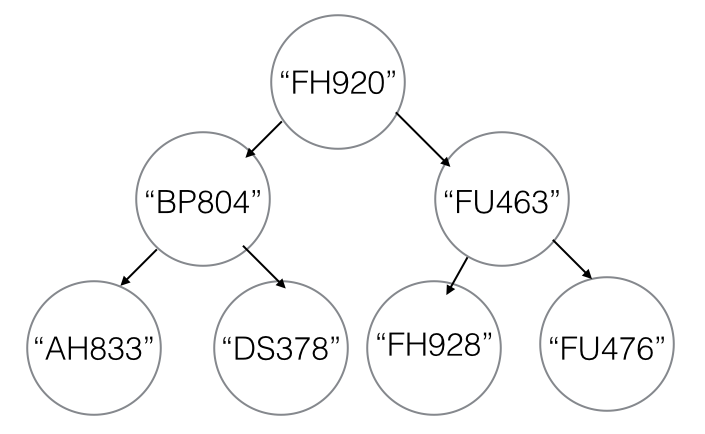
\includegraphics[width=90mm]{catclientes.png}
\caption{Exemplo de um TreeSet de clientes}
\end{figure}

\newpage
\subsection{Catálogo de Produtos}
\par O catálogo de clientes foi implementado usando a class  \textbf{ProductsCatalog} que basicamente guarda os códigos
dos produtos num TreeSet. Como os códigos dos produtos são apenas \textbf{String} a árvore fica então ordenada
alfabeticamente e a procura é rápida.

\begin{figure}[ht!]
\centering
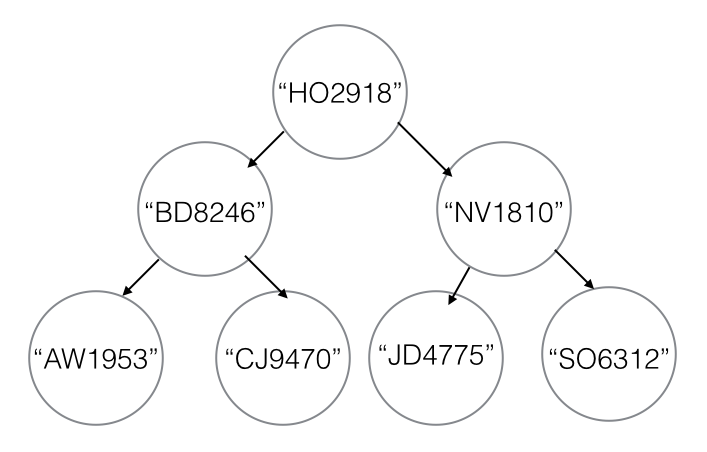
\includegraphics[width=90mm]{catprodutos.png}
\caption{Exemplo de um TreeSet de produtos}
\label{fig:catprodutos}
\end{figure}

\subsection{Compras}
\par O módulo de compras é responsável por guardar todas as compras válidas, relacionando quais os clientes que fizeram
essas compras e quando, para ser possivel consultar as vendas por mês se assim for desejado.
\par Como então era necessário conseguir dividir as compras por mês utilizamos um \textbf{ArrayList} com 12 entradas, e
em cada uma destas entradas existe um \textbf{TreeMap\textless String, ArrayList\textless Sale\textgreater\textgreater} que
mapeia um código de cliente para a lista de compras efectuadas por esse cliente. Usando um \textbf{TreeMap} permite uma
procura rápida por um dado cliente e o arraylist permite um acesso directo ás compras de um determinado mês.
\par A declaração das variáveis de instância é a seguinte:

\begin{lstlisting}[language=Java]
public class Sales {
	ArrayList<TreeMap<String, ArrayList<Sale>>> sales;
	...
}
\end{lstlisting}

\par Para mais facilmente entender a implementação incluimos uma figura da estrutura:

\begin{figure}[ht!]
\centering
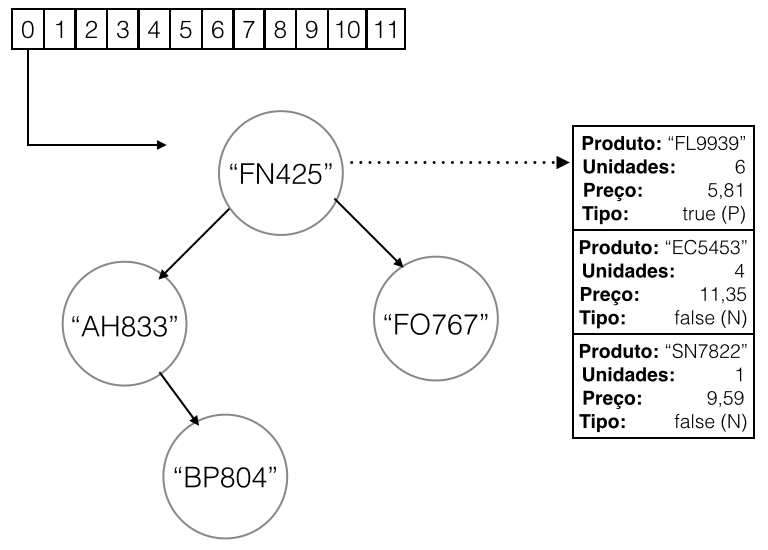
\includegraphics[width=90mm]{sales.png}
\caption{Exemplo da estrutura com as compras de Janeiro do cliente "FN425"}
\label{fig:sales}
\end{figure}

% UI
\newpage
\section{Interface Utilizador}

\newpage
\section{Diagrama de Classes}

\newpage
\section{Gráficos e Resultados}

\newpage
\section{Conclusão}

\end{document}